% Created by tikzDevice version 0.12.6 on 2024-03-15 15:16:56
% !TEX encoding = UTF-8 Unicode
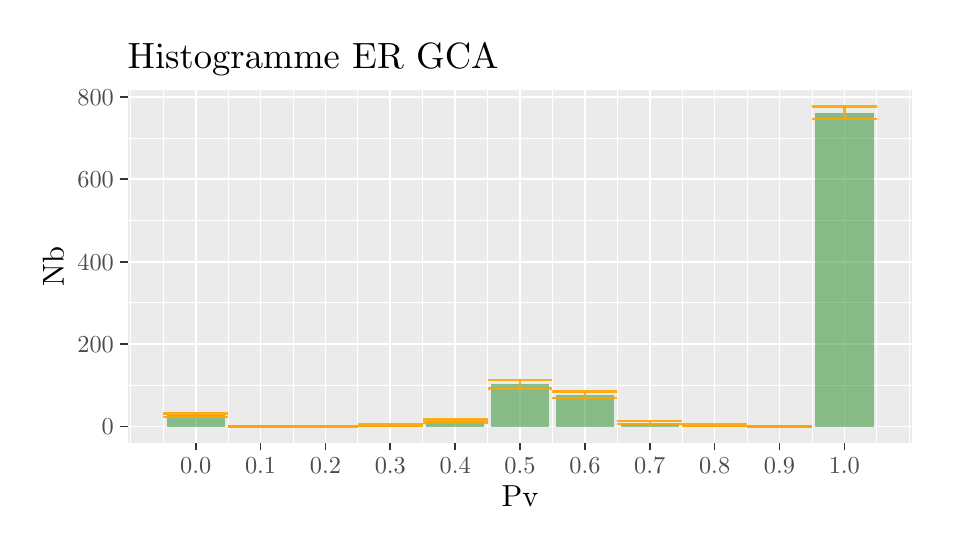
\begin{tikzpicture}[x=1pt,y=1pt]
\definecolor{fillColor}{RGB}{255,255,255}
\path[use as bounding box,fill=fillColor,fill opacity=0.00] (0,0) rectangle (325.21,180.67);
\begin{scope}
\path[clip] (  0.00,  0.00) rectangle (325.21,180.67);
\definecolor{drawColor}{RGB}{255,255,255}
\definecolor{fillColor}{RGB}{255,255,255}

\path[draw=drawColor,line width= 0.6pt,line join=round,line cap=round,fill=fillColor] (  0.00,  0.00) rectangle (325.21,180.68);
\end{scope}
\begin{scope}
\path[clip] ( 36.11, 30.69) rectangle (319.71,158.02);
\definecolor{fillColor}{gray}{0.92}

\path[fill=fillColor] ( 36.11, 30.69) rectangle (319.71,158.02);
\definecolor{drawColor}{RGB}{255,255,255}

\path[draw=drawColor,line width= 0.3pt,line join=round] ( 36.11, 51.41) --
	(319.71, 51.41);

\path[draw=drawColor,line width= 0.3pt,line join=round] ( 36.11, 81.21) --
	(319.71, 81.21);

\path[draw=drawColor,line width= 0.3pt,line join=round] ( 36.11,111.00) --
	(319.71,111.00);

\path[draw=drawColor,line width= 0.3pt,line join=round] ( 36.11,140.79) --
	(319.71,140.79);

\path[draw=drawColor,line width= 0.3pt,line join=round] ( 37.28, 30.69) --
	( 37.28,158.02);

\path[draw=drawColor,line width= 0.3pt,line join=round] ( 49.00, 30.69) --
	( 49.00,158.02);

\path[draw=drawColor,line width= 0.3pt,line join=round] ( 72.44, 30.69) --
	( 72.44,158.02);

\path[draw=drawColor,line width= 0.3pt,line join=round] ( 95.88, 30.69) --
	( 95.88,158.02);

\path[draw=drawColor,line width= 0.3pt,line join=round] (119.32, 30.69) --
	(119.32,158.02);

\path[draw=drawColor,line width= 0.3pt,line join=round] (142.76, 30.69) --
	(142.76,158.02);

\path[draw=drawColor,line width= 0.3pt,line join=round] (166.19, 30.69) --
	(166.19,158.02);

\path[draw=drawColor,line width= 0.3pt,line join=round] (189.63, 30.69) --
	(189.63,158.02);

\path[draw=drawColor,line width= 0.3pt,line join=round] (213.07, 30.69) --
	(213.07,158.02);

\path[draw=drawColor,line width= 0.3pt,line join=round] (236.51, 30.69) --
	(236.51,158.02);

\path[draw=drawColor,line width= 0.3pt,line join=round] (259.95, 30.69) --
	(259.95,158.02);

\path[draw=drawColor,line width= 0.3pt,line join=round] (283.39, 30.69) --
	(283.39,158.02);

\path[draw=drawColor,line width= 0.3pt,line join=round] (306.82, 30.69) --
	(306.82,158.02);

\path[draw=drawColor,line width= 0.3pt,line join=round] (318.54, 30.69) --
	(318.54,158.02);

\path[draw=drawColor,line width= 0.6pt,line join=round] ( 36.11, 36.52) --
	(319.71, 36.52);

\path[draw=drawColor,line width= 0.6pt,line join=round] ( 36.11, 66.31) --
	(319.71, 66.31);

\path[draw=drawColor,line width= 0.6pt,line join=round] ( 36.11, 96.10) --
	(319.71, 96.10);

\path[draw=drawColor,line width= 0.6pt,line join=round] ( 36.11,125.89) --
	(319.71,125.89);

\path[draw=drawColor,line width= 0.6pt,line join=round] ( 36.11,155.69) --
	(319.71,155.69);

\path[draw=drawColor,line width= 0.6pt,line join=round] ( 60.72, 30.69) --
	( 60.72,158.02);

\path[draw=drawColor,line width= 0.6pt,line join=round] ( 84.16, 30.69) --
	( 84.16,158.02);

\path[draw=drawColor,line width= 0.6pt,line join=round] (107.60, 30.69) --
	(107.60,158.02);

\path[draw=drawColor,line width= 0.6pt,line join=round] (131.04, 30.69) --
	(131.04,158.02);

\path[draw=drawColor,line width= 0.6pt,line join=round] (154.47, 30.69) --
	(154.47,158.02);

\path[draw=drawColor,line width= 0.6pt,line join=round] (177.91, 30.69) --
	(177.91,158.02);

\path[draw=drawColor,line width= 0.6pt,line join=round] (201.35, 30.69) --
	(201.35,158.02);

\path[draw=drawColor,line width= 0.6pt,line join=round] (224.79, 30.69) --
	(224.79,158.02);

\path[draw=drawColor,line width= 0.6pt,line join=round] (248.23, 30.69) --
	(248.23,158.02);

\path[draw=drawColor,line width= 0.6pt,line join=round] (271.67, 30.69) --
	(271.67,158.02);

\path[draw=drawColor,line width= 0.6pt,line join=round] (295.10, 30.69) --
	(295.10,158.02);
\definecolor{fillColor}{RGB}{34,139,34}

\path[fill=fillColor,fill opacity=0.50] ( 50.17, 36.52) rectangle ( 71.27, 40.62);

\path[fill=fillColor,fill opacity=0.50] ( 73.61, 36.52) rectangle ( 94.71, 36.52);

\path[fill=fillColor,fill opacity=0.50] ( 97.05, 36.52) rectangle (118.15, 36.59);

\path[fill=fillColor,fill opacity=0.50] (120.49, 36.52) rectangle (141.58, 37.09);

\path[fill=fillColor,fill opacity=0.50] (143.93, 36.52) rectangle (165.02, 38.53);

\path[fill=fillColor,fill opacity=0.50] (167.37, 36.52) rectangle (188.46, 51.88);

\path[fill=fillColor,fill opacity=0.50] (190.80, 36.52) rectangle (211.90, 48.04);

\path[fill=fillColor,fill opacity=0.50] (214.24, 36.52) rectangle (235.34, 37.94);

\path[fill=fillColor,fill opacity=0.50] (237.68, 36.52) rectangle (258.78, 36.93);

\path[fill=fillColor,fill opacity=0.50] (261.12, 36.52) rectangle (282.21, 36.56);

\path[fill=fillColor,fill opacity=0.50] (284.56, 36.52) rectangle (305.65,149.95);
\definecolor{drawColor}{RGB}{255,165,0}

\path[draw=drawColor,draw opacity=0.90,line width= 0.9pt,line join=round] ( 49.00, 41.33) --
	( 72.44, 41.33);

\path[draw=drawColor,draw opacity=0.90,line width= 0.9pt,line join=round] ( 60.72, 41.33) --
	( 60.72, 39.92);

\path[draw=drawColor,draw opacity=0.90,line width= 0.9pt,line join=round] ( 49.00, 39.92) --
	( 72.44, 39.92);

\path[draw=drawColor,draw opacity=0.90,line width= 0.9pt,line join=round] ( 72.44, 36.54) --
	( 95.88, 36.54);

\path[draw=drawColor,draw opacity=0.90,line width= 0.9pt,line join=round] ( 84.16, 36.54) --
	( 84.16, 36.50);

\path[draw=drawColor,draw opacity=0.90,line width= 0.9pt,line join=round] ( 72.44, 36.50) --
	( 95.88, 36.50);

\path[draw=drawColor,draw opacity=0.90,line width= 0.9pt,line join=round] ( 95.88, 36.69) --
	(119.32, 36.69);

\path[draw=drawColor,draw opacity=0.90,line width= 0.9pt,line join=round] (107.60, 36.69) --
	(107.60, 36.49);

\path[draw=drawColor,draw opacity=0.90,line width= 0.9pt,line join=round] ( 95.88, 36.49) --
	(119.32, 36.49);

\path[draw=drawColor,draw opacity=0.90,line width= 0.9pt,line join=round] (119.32, 37.40) --
	(142.76, 37.40);

\path[draw=drawColor,draw opacity=0.90,line width= 0.9pt,line join=round] (131.04, 37.40) --
	(131.04, 36.78);

\path[draw=drawColor,draw opacity=0.90,line width= 0.9pt,line join=round] (119.32, 36.78) --
	(142.76, 36.78);

\path[draw=drawColor,draw opacity=0.90,line width= 0.9pt,line join=round] (142.76, 39.10) --
	(166.19, 39.10);

\path[draw=drawColor,draw opacity=0.90,line width= 0.9pt,line join=round] (154.47, 39.10) --
	(154.47, 37.96);

\path[draw=drawColor,draw opacity=0.90,line width= 0.9pt,line join=round] (142.76, 37.96) --
	(166.19, 37.96);

\path[draw=drawColor,draw opacity=0.90,line width= 0.9pt,line join=round] (166.19, 53.40) --
	(189.63, 53.40);

\path[draw=drawColor,draw opacity=0.90,line width= 0.9pt,line join=round] (177.91, 53.40) --
	(177.91, 50.36);

\path[draw=drawColor,draw opacity=0.90,line width= 0.9pt,line join=round] (166.19, 50.36) --
	(189.63, 50.36);

\path[draw=drawColor,draw opacity=0.90,line width= 0.9pt,line join=round] (189.63, 49.16) --
	(213.07, 49.16);

\path[draw=drawColor,draw opacity=0.90,line width= 0.9pt,line join=round] (201.35, 49.16) --
	(201.35, 46.93);

\path[draw=drawColor,draw opacity=0.90,line width= 0.9pt,line join=round] (189.63, 46.93) --
	(213.07, 46.93);

\path[draw=drawColor,draw opacity=0.90,line width= 0.9pt,line join=round] (213.07, 38.47) --
	(236.51, 38.47);

\path[draw=drawColor,draw opacity=0.90,line width= 0.9pt,line join=round] (224.79, 38.47) --
	(224.79, 37.41);

\path[draw=drawColor,draw opacity=0.90,line width= 0.9pt,line join=round] (213.07, 37.41) --
	(236.51, 37.41);

\path[draw=drawColor,draw opacity=0.90,line width= 0.9pt,line join=round] (236.51, 37.19) --
	(259.95, 37.19);

\path[draw=drawColor,draw opacity=0.90,line width= 0.9pt,line join=round] (248.23, 37.19) --
	(248.23, 36.67);

\path[draw=drawColor,draw opacity=0.90,line width= 0.9pt,line join=round] (236.51, 36.67) --
	(259.95, 36.67);

\path[draw=drawColor,draw opacity=0.90,line width= 0.9pt,line join=round] (259.95, 36.64) --
	(283.39, 36.64);

\path[draw=drawColor,draw opacity=0.90,line width= 0.9pt,line join=round] (271.67, 36.64) --
	(271.67, 36.47);

\path[draw=drawColor,draw opacity=0.90,line width= 0.9pt,line join=round] (259.95, 36.47) --
	(283.39, 36.47);

\path[draw=drawColor,draw opacity=0.90,line width= 0.9pt,line join=round] (283.39,152.23) --
	(306.82,152.23);

\path[draw=drawColor,draw opacity=0.90,line width= 0.9pt,line join=round] (295.10,152.23) --
	(295.10,147.67);

\path[draw=drawColor,draw opacity=0.90,line width= 0.9pt,line join=round] (283.39,147.67) --
	(306.82,147.67);
\end{scope}
\begin{scope}
\path[clip] (  0.00,  0.00) rectangle (325.21,180.67);
\definecolor{drawColor}{gray}{0.30}

\node[text=drawColor,anchor=base east,inner sep=0pt, outer sep=0pt, scale=  0.88] at ( 31.16, 33.49) {0};

\node[text=drawColor,anchor=base east,inner sep=0pt, outer sep=0pt, scale=  0.88] at ( 31.16, 63.28) {200};

\node[text=drawColor,anchor=base east,inner sep=0pt, outer sep=0pt, scale=  0.88] at ( 31.16, 93.07) {400};

\node[text=drawColor,anchor=base east,inner sep=0pt, outer sep=0pt, scale=  0.88] at ( 31.16,122.86) {600};

\node[text=drawColor,anchor=base east,inner sep=0pt, outer sep=0pt, scale=  0.88] at ( 31.16,152.66) {800};
\end{scope}
\begin{scope}
\path[clip] (  0.00,  0.00) rectangle (325.21,180.67);
\definecolor{drawColor}{gray}{0.20}

\path[draw=drawColor,line width= 0.6pt,line join=round] ( 33.36, 36.52) --
	( 36.11, 36.52);

\path[draw=drawColor,line width= 0.6pt,line join=round] ( 33.36, 66.31) --
	( 36.11, 66.31);

\path[draw=drawColor,line width= 0.6pt,line join=round] ( 33.36, 96.10) --
	( 36.11, 96.10);

\path[draw=drawColor,line width= 0.6pt,line join=round] ( 33.36,125.89) --
	( 36.11,125.89);

\path[draw=drawColor,line width= 0.6pt,line join=round] ( 33.36,155.69) --
	( 36.11,155.69);
\end{scope}
\begin{scope}
\path[clip] (  0.00,  0.00) rectangle (325.21,180.67);
\definecolor{drawColor}{gray}{0.20}

\path[draw=drawColor,line width= 0.6pt,line join=round] ( 60.72, 27.94) --
	( 60.72, 30.69);

\path[draw=drawColor,line width= 0.6pt,line join=round] ( 84.16, 27.94) --
	( 84.16, 30.69);

\path[draw=drawColor,line width= 0.6pt,line join=round] (107.60, 27.94) --
	(107.60, 30.69);

\path[draw=drawColor,line width= 0.6pt,line join=round] (131.04, 27.94) --
	(131.04, 30.69);

\path[draw=drawColor,line width= 0.6pt,line join=round] (154.47, 27.94) --
	(154.47, 30.69);

\path[draw=drawColor,line width= 0.6pt,line join=round] (177.91, 27.94) --
	(177.91, 30.69);

\path[draw=drawColor,line width= 0.6pt,line join=round] (201.35, 27.94) --
	(201.35, 30.69);

\path[draw=drawColor,line width= 0.6pt,line join=round] (224.79, 27.94) --
	(224.79, 30.69);

\path[draw=drawColor,line width= 0.6pt,line join=round] (248.23, 27.94) --
	(248.23, 30.69);

\path[draw=drawColor,line width= 0.6pt,line join=round] (271.67, 27.94) --
	(271.67, 30.69);

\path[draw=drawColor,line width= 0.6pt,line join=round] (295.10, 27.94) --
	(295.10, 30.69);
\end{scope}
\begin{scope}
\path[clip] (  0.00,  0.00) rectangle (325.21,180.67);
\definecolor{drawColor}{gray}{0.30}

\node[text=drawColor,anchor=base,inner sep=0pt, outer sep=0pt, scale=  0.88] at ( 60.72, 19.68) {0.0};

\node[text=drawColor,anchor=base,inner sep=0pt, outer sep=0pt, scale=  0.88] at ( 84.16, 19.68) {0.1};

\node[text=drawColor,anchor=base,inner sep=0pt, outer sep=0pt, scale=  0.88] at (107.60, 19.68) {0.2};

\node[text=drawColor,anchor=base,inner sep=0pt, outer sep=0pt, scale=  0.88] at (131.04, 19.68) {0.3};

\node[text=drawColor,anchor=base,inner sep=0pt, outer sep=0pt, scale=  0.88] at (154.47, 19.68) {0.4};

\node[text=drawColor,anchor=base,inner sep=0pt, outer sep=0pt, scale=  0.88] at (177.91, 19.68) {0.5};

\node[text=drawColor,anchor=base,inner sep=0pt, outer sep=0pt, scale=  0.88] at (201.35, 19.68) {0.6};

\node[text=drawColor,anchor=base,inner sep=0pt, outer sep=0pt, scale=  0.88] at (224.79, 19.68) {0.7};

\node[text=drawColor,anchor=base,inner sep=0pt, outer sep=0pt, scale=  0.88] at (248.23, 19.68) {0.8};

\node[text=drawColor,anchor=base,inner sep=0pt, outer sep=0pt, scale=  0.88] at (271.67, 19.68) {0.9};

\node[text=drawColor,anchor=base,inner sep=0pt, outer sep=0pt, scale=  0.88] at (295.10, 19.68) {1.0};
\end{scope}
\begin{scope}
\path[clip] (  0.00,  0.00) rectangle (325.21,180.67);
\definecolor{drawColor}{RGB}{0,0,0}

\node[text=drawColor,anchor=base,inner sep=0pt, outer sep=0pt, scale=  1.10] at (177.91,  7.64) {Pv};
\end{scope}
\begin{scope}
\path[clip] (  0.00,  0.00) rectangle (325.21,180.67);
\definecolor{drawColor}{RGB}{0,0,0}

\node[text=drawColor,rotate= 90.00,anchor=base,inner sep=0pt, outer sep=0pt, scale=  1.10] at ( 13.08, 94.35) {Nb};
\end{scope}
\begin{scope}
\path[clip] (  0.00,  0.00) rectangle (325.21,180.67);
\definecolor{drawColor}{RGB}{0,0,0}

\node[text=drawColor,anchor=base west,inner sep=0pt, outer sep=0pt, scale=  1.32] at ( 36.11,166.08) {Histogramme ER GCA};
\end{scope}
\end{tikzpicture}
